% Self-contained section on overclocking past STA timing closure.
% % Self-contained section on overclocking past STA timing closure.
% % Self-contained section on overclocking past STA timing closure.
% % Self-contained section on overclocking past STA timing closure.
% \input{overclocking_section} into alife-lbw.tex (note: pushes past 2pp; see notes).
% Numbers as \PLACEHOLDER... are backfilled from the measured sweep.

\section{Overclocking Past Timing Closure}

An FPGA place-and-route tool reports a maximum clock from \emph{static timing
analysis} (STA): a conservative bound at a worst-case process/voltage/temperature
corner. It is a prediction, not a measurement --- and the LiteX/trellis flow
emits a bitstream even when a requested clock \emph{violates} it. We test what the
real silicon does past the bound. A per-build clock override (one PLL parameter,
exposed as a submission argument) sets the SoC compute-clock; the Ethernet domain
is fixed by the RMII PHY, so only the compute fabric is reclocked. We sweep it,
build, flash, and run on real ECP5-85 boards, checking functional correctness and
throughput.

\begin{figure}[t]
    \centering
    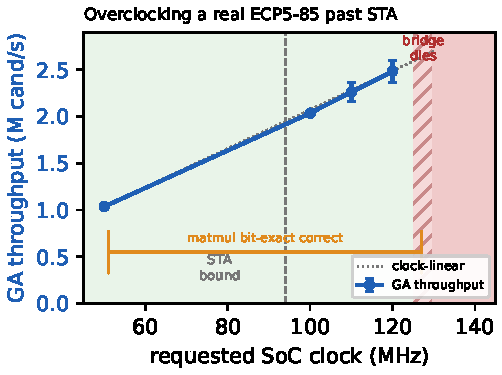
\includegraphics[width=\columnwidth]{figures/fig_overclock.pdf}
    \caption{Overclocking the $K{=}16$ engine on a real ECP5-85. STA predicts
    $\sim$94\,MHz, but the design runs correct and throughput scales to
    120\,MHz; a bit-exact matmul probe is error-free through 128\,MHz. The hard
    limit ($\sim$125--130\,MHz, marginal) is the soft-CPU control bridge, not the
    datapath.}
    \label{fig:overclock}
\end{figure}

\textbf{Silicon beats the model by a wide margin} (\Cref{fig:overclock}). STA
predicts the $K{=}16$ engine tops out at \mbox{$\sim$94\,MHz}. On hardware at
room temperature it \emph{solves the target and scales} well past that: \mbox{$\sim$2.0\,M\,cand/s}
at 100\,MHz ($2\times$ the 50\,MHz default) and \mbox{$2.48{\pm}0.12$\,M\,cand/s}
at 120\,MHz (mean of 6 runs, all solving) --- \mbox{$\sim$28\%} beyond STA, a
\mbox{$2.4\times$} gain that \emph{exceeds a full Apple M4} (2.42\,M/s) with 16
cores on a \mbox{$\sim$\$40} part, all correct. To probe correctness directly we ran a
bit-exact arithmetic kernel (a 4$\times$4 signed matrix multiply, real MAC logic)
over many random inputs against a software reference: it is \textbf{bit-exact
correct at every clock the board responds to, through 128\,MHz}
($\sim$750 multiplies, zero element errors) --- $\sim$36\% past STA. The
tool's bound is \emph{very} conservative; a large band of real, usable frequency
sits above it.

\textbf{The bottleneck is the control bridge, not the accelerator.} The hard
limit is not the compute fabric. Around \mbox{125--130\,MHz} the board goes
\emph{unresponsive} --- the bitstream still programs, but the soft
VexRiscv\,+\,LiteEth bridge can no longer service packets --- and this failure is
\emph{marginal and probabilistic}: a 125\,MHz build died after 11 transactions
while a 128\,MHz build completed 150, the run-to-run luck expected right at a
timing edge. So the accelerator's arithmetic never produces a wrong answer in the
entire usable range; the \emph{control processor} fails first. The actionable
implication is that the path to more headroom is a hardened or minimal control
plane (e.g.\ a hardware Etherbone bridge replacing the soft CPU), not a faster
datapath.

\textbf{Implications for evolutionary hardware.} The immediate, demonstrated win
is concrete: a one-line clock change buys a measured \mbox{$\sim$2$\times$}
throughput at fully correct results, because the conservative STA bound hides
that much real margin. The deeper, and we think more interesting, question is
whether evolutionary workloads can exploit the regime \emph{past} clean
correctness --- where the compute itself starts to miss timing and produce silent
errors. There is reason to expect they can: an evolutionary search is already a
stochastic process that draws mostly-unfit candidates and selects the rare good
ones, so a corrupted evaluation is one more noisy sample in a pipeline built to
tolerate noise (errors do not accumulate; a wrongly-rejected candidate is
replaced by the next draw, a wrongly-promoted one selected against on
re-evaluation). This places evolutionary hardware in the lineage of approximate
computing and of intrinsic evolvable hardware \citep{thompson1996evolved}, which
exploited the analog physics of real silicon --- here the exploitable physics is
timing margin. Yet on this chip we never reach that regime: the engine's
throughput stays \emph{clock-linear} with no measurable deficit through
120\,MHz (within the $\sim$5\% run-to-run noise; 6 of 6 runs solve at both 110
and 120), and the matmul probe is exact to 128. The compute simply does not err
before \emph{the control bridge fails first}. So the error-tolerance hypothesis,
though well-motivated, is untested here; confirming it as a usable throughput
lever is gated on first removing the bridge bottleneck to expose the datapath's
own error regime --- a concrete next experiment.

\textbf{Caveats.} Results are one device at one temperature; timing margins and
the exact failure clock vary with both. The error-tolerance argument requires
\emph{selection} --- a pure random search that trusts a single best-fitness read
is vulnerable to a false positive from a scoring error, whereas a re-evaluating
GA is not. Achieved-Fmax and a timing-met flag, surfaced per build, would make
the clean/degraded boundary visible to users rather than inferred.
 into alife-lbw.tex (note: pushes past 2pp; see notes).
% Numbers as \PLACEHOLDER... are backfilled from the measured sweep.

\section{Overclocking Past Timing Closure}

An FPGA place-and-route tool reports a maximum clock from \emph{static timing
analysis} (STA): a conservative bound at a worst-case process/voltage/temperature
corner. It is a prediction, not a measurement --- and the LiteX/trellis flow
emits a bitstream even when a requested clock \emph{violates} it. We test what the
real silicon does past the bound. A per-build clock override (one PLL parameter,
exposed as a submission argument) sets the SoC compute-clock; the Ethernet domain
is fixed by the RMII PHY, so only the compute fabric is reclocked. We sweep it,
build, flash, and run on real ECP5-85 boards, checking functional correctness and
throughput.

\begin{figure}[t]
    \centering
    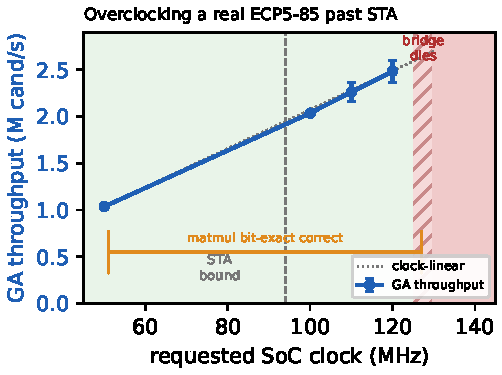
\includegraphics[width=\columnwidth]{figures/fig_overclock.pdf}
    \caption{Overclocking the $K{=}16$ engine on a real ECP5-85. STA predicts
    $\sim$94\,MHz, but the design runs correct and throughput scales to
    120\,MHz; a bit-exact matmul probe is error-free through 128\,MHz. The hard
    limit ($\sim$125--130\,MHz, marginal) is the soft-CPU control bridge, not the
    datapath.}
    \label{fig:overclock}
\end{figure}

\textbf{Silicon beats the model by a wide margin} (\Cref{fig:overclock}). STA
predicts the $K{=}16$ engine tops out at \mbox{$\sim$94\,MHz}. On hardware at
room temperature it \emph{solves the target and scales} well past that: \mbox{$\sim$2.0\,M\,cand/s}
at 100\,MHz ($2\times$ the 50\,MHz default) and \mbox{$2.48{\pm}0.12$\,M\,cand/s}
at 120\,MHz (mean of 6 runs, all solving) --- \mbox{$\sim$28\%} beyond STA, a
\mbox{$2.4\times$} gain that \emph{exceeds a full Apple M4} (2.42\,M/s) with 16
cores on a \mbox{$\sim$\$40} part, all correct. To probe correctness directly we ran a
bit-exact arithmetic kernel (a 4$\times$4 signed matrix multiply, real MAC logic)
over many random inputs against a software reference: it is \textbf{bit-exact
correct at every clock the board responds to, through 128\,MHz}
($\sim$750 multiplies, zero element errors) --- $\sim$36\% past STA. The
tool's bound is \emph{very} conservative; a large band of real, usable frequency
sits above it.

\textbf{The bottleneck is the control bridge, not the accelerator.} The hard
limit is not the compute fabric. Around \mbox{125--130\,MHz} the board goes
\emph{unresponsive} --- the bitstream still programs, but the soft
VexRiscv\,+\,LiteEth bridge can no longer service packets --- and this failure is
\emph{marginal and probabilistic}: a 125\,MHz build died after 11 transactions
while a 128\,MHz build completed 150, the run-to-run luck expected right at a
timing edge. So the accelerator's arithmetic never produces a wrong answer in the
entire usable range; the \emph{control processor} fails first. The actionable
implication is that the path to more headroom is a hardened or minimal control
plane (e.g.\ a hardware Etherbone bridge replacing the soft CPU), not a faster
datapath.

\textbf{Implications for evolutionary hardware.} The immediate, demonstrated win
is concrete: a one-line clock change buys a measured \mbox{$\sim$2$\times$}
throughput at fully correct results, because the conservative STA bound hides
that much real margin. The deeper, and we think more interesting, question is
whether evolutionary workloads can exploit the regime \emph{past} clean
correctness --- where the compute itself starts to miss timing and produce silent
errors. There is reason to expect they can: an evolutionary search is already a
stochastic process that draws mostly-unfit candidates and selects the rare good
ones, so a corrupted evaluation is one more noisy sample in a pipeline built to
tolerate noise (errors do not accumulate; a wrongly-rejected candidate is
replaced by the next draw, a wrongly-promoted one selected against on
re-evaluation). This places evolutionary hardware in the lineage of approximate
computing and of intrinsic evolvable hardware \citep{thompson1996evolved}, which
exploited the analog physics of real silicon --- here the exploitable physics is
timing margin. Yet on this chip we never reach that regime: the engine's
throughput stays \emph{clock-linear} with no measurable deficit through
120\,MHz (within the $\sim$5\% run-to-run noise; 6 of 6 runs solve at both 110
and 120), and the matmul probe is exact to 128. The compute simply does not err
before \emph{the control bridge fails first}. So the error-tolerance hypothesis,
though well-motivated, is untested here; confirming it as a usable throughput
lever is gated on first removing the bridge bottleneck to expose the datapath's
own error regime --- a concrete next experiment.

\textbf{Caveats.} Results are one device at one temperature; timing margins and
the exact failure clock vary with both. The error-tolerance argument requires
\emph{selection} --- a pure random search that trusts a single best-fitness read
is vulnerable to a false positive from a scoring error, whereas a re-evaluating
GA is not. Achieved-Fmax and a timing-met flag, surfaced per build, would make
the clean/degraded boundary visible to users rather than inferred.
 into alife-lbw.tex (note: pushes past 2pp; see notes).
% Numbers as \PLACEHOLDER... are backfilled from the measured sweep.

\section{Overclocking Past Timing Closure}

An FPGA place-and-route tool reports a maximum clock from \emph{static timing
analysis} (STA): a conservative bound at a worst-case process/voltage/temperature
corner. It is a prediction, not a measurement --- and the LiteX/trellis flow
emits a bitstream even when a requested clock \emph{violates} it. We test what the
real silicon does past the bound. A per-build clock override (one PLL parameter,
exposed as a submission argument) sets the SoC compute-clock; the Ethernet domain
is fixed by the RMII PHY, so only the compute fabric is reclocked. We sweep it,
build, flash, and run on real ECP5-85 boards, checking functional correctness and
throughput.

\begin{figure}[t]
    \centering
    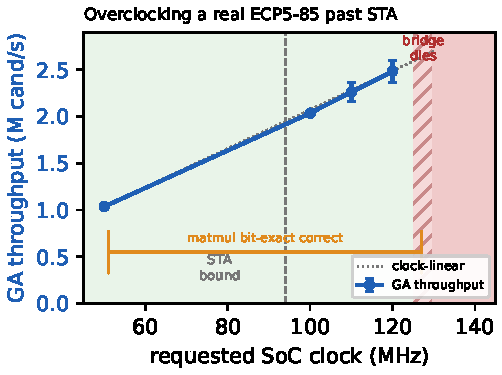
\includegraphics[width=\columnwidth]{figures/fig_overclock.pdf}
    \caption{Overclocking the $K{=}16$ engine on a real ECP5-85. STA predicts
    $\sim$94\,MHz, but the design runs correct and throughput scales to
    120\,MHz; a bit-exact matmul probe is error-free through 128\,MHz. The hard
    limit ($\sim$125--130\,MHz, marginal) is the soft-CPU control bridge, not the
    datapath.}
    \label{fig:overclock}
\end{figure}

\textbf{Silicon beats the model by a wide margin} (\Cref{fig:overclock}). STA
predicts the $K{=}16$ engine tops out at \mbox{$\sim$94\,MHz}. On hardware at
room temperature it \emph{solves the target and scales} well past that: \mbox{$\sim$2.0\,M\,cand/s}
at 100\,MHz ($2\times$ the 50\,MHz default) and \mbox{$2.48{\pm}0.12$\,M\,cand/s}
at 120\,MHz (mean of 6 runs, all solving) --- \mbox{$\sim$28\%} beyond STA, a
\mbox{$2.4\times$} gain that \emph{exceeds a full Apple M4} (2.42\,M/s) with 16
cores on a \mbox{$\sim$\$40} part, all correct. To probe correctness directly we ran a
bit-exact arithmetic kernel (a 4$\times$4 signed matrix multiply, real MAC logic)
over many random inputs against a software reference: it is \textbf{bit-exact
correct at every clock the board responds to, through 128\,MHz}
($\sim$750 multiplies, zero element errors) --- $\sim$36\% past STA. The
tool's bound is \emph{very} conservative; a large band of real, usable frequency
sits above it.

\textbf{The bottleneck is the control bridge, not the accelerator.} The hard
limit is not the compute fabric. Around \mbox{125--130\,MHz} the board goes
\emph{unresponsive} --- the bitstream still programs, but the soft
VexRiscv\,+\,LiteEth bridge can no longer service packets --- and this failure is
\emph{marginal and probabilistic}: a 125\,MHz build died after 11 transactions
while a 128\,MHz build completed 150, the run-to-run luck expected right at a
timing edge. So the accelerator's arithmetic never produces a wrong answer in the
entire usable range; the \emph{control processor} fails first. The actionable
implication is that the path to more headroom is a hardened or minimal control
plane (e.g.\ a hardware Etherbone bridge replacing the soft CPU), not a faster
datapath.

\textbf{Implications for evolutionary hardware.} The immediate, demonstrated win
is concrete: a one-line clock change buys a measured \mbox{$\sim$2$\times$}
throughput at fully correct results, because the conservative STA bound hides
that much real margin. The deeper, and we think more interesting, question is
whether evolutionary workloads can exploit the regime \emph{past} clean
correctness --- where the compute itself starts to miss timing and produce silent
errors. There is reason to expect they can: an evolutionary search is already a
stochastic process that draws mostly-unfit candidates and selects the rare good
ones, so a corrupted evaluation is one more noisy sample in a pipeline built to
tolerate noise (errors do not accumulate; a wrongly-rejected candidate is
replaced by the next draw, a wrongly-promoted one selected against on
re-evaluation). This places evolutionary hardware in the lineage of approximate
computing and of intrinsic evolvable hardware \citep{thompson1996evolved}, which
exploited the analog physics of real silicon --- here the exploitable physics is
timing margin. Yet on this chip we never reach that regime: the engine's
throughput stays \emph{clock-linear} with no measurable deficit through
120\,MHz (within the $\sim$5\% run-to-run noise; 6 of 6 runs solve at both 110
and 120), and the matmul probe is exact to 128. The compute simply does not err
before \emph{the control bridge fails first}. So the error-tolerance hypothesis,
though well-motivated, is untested here; confirming it as a usable throughput
lever is gated on first removing the bridge bottleneck to expose the datapath's
own error regime --- a concrete next experiment.

\textbf{Caveats.} Results are one device at one temperature; timing margins and
the exact failure clock vary with both. The error-tolerance argument requires
\emph{selection} --- a pure random search that trusts a single best-fitness read
is vulnerable to a false positive from a scoring error, whereas a re-evaluating
GA is not. Achieved-Fmax and a timing-met flag, surfaced per build, would make
the clean/degraded boundary visible to users rather than inferred.
 into alife-lbw.tex (note: pushes past 2pp; see notes).
% Numbers as \PLACEHOLDER... are backfilled from the measured sweep.

\section{Overclocking Past Timing Closure}

An FPGA place-and-route tool reports a maximum clock from \emph{static timing
analysis} (STA): a conservative bound at a worst-case process/voltage/temperature
corner. It is a prediction, not a measurement --- and the LiteX/trellis flow
emits a bitstream even when a requested clock \emph{violates} it. We test what the
real silicon does past the bound. A per-build clock override (one PLL parameter,
exposed as a submission argument) sets the SoC compute-clock; the Ethernet domain
is fixed by the RMII PHY, so only the compute fabric is reclocked. We sweep it,
build, flash, and run on real ECP5-85 boards, checking functional correctness and
throughput.

\begin{figure}[t]
    \centering
    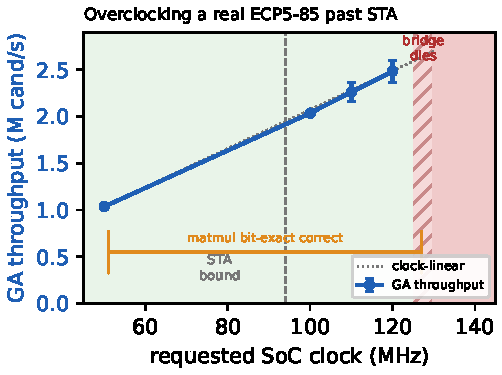
\includegraphics[width=\columnwidth]{figures/fig_overclock.pdf}
    \caption{Overclocking the $K{=}16$ engine on a real ECP5-85. STA predicts
    $\sim$94\,MHz, but the design runs correct and throughput scales to
    120\,MHz; a bit-exact matmul probe is error-free through 128\,MHz. The hard
    limit ($\sim$125--130\,MHz, marginal) is the soft-CPU control bridge, not the
    datapath.}
    \label{fig:overclock}
\end{figure}

\textbf{Silicon beats the model by a wide margin} (\Cref{fig:overclock}). STA
predicts the $K{=}16$ engine tops out at \mbox{$\sim$94\,MHz}. On hardware at
room temperature it \emph{solves the target and scales} well past that: \mbox{$\sim$2.0\,M\,cand/s}
at 100\,MHz ($2\times$ the 50\,MHz default) and \mbox{$2.48{\pm}0.12$\,M\,cand/s}
at 120\,MHz (mean of 6 runs, all solving) --- \mbox{$\sim$28\%} beyond STA, a
\mbox{$2.4\times$} gain that \emph{exceeds a full Apple M4} (2.42\,M/s) with 16
cores on a \mbox{$\sim$\$40} part, all correct. To probe correctness directly we ran a
bit-exact arithmetic kernel (a 4$\times$4 signed matrix multiply, real MAC logic)
over many random inputs against a software reference: it is \textbf{bit-exact
correct at every clock the board responds to, through 128\,MHz}
($\sim$750 multiplies, zero element errors) --- $\sim$36\% past STA. The
tool's bound is \emph{very} conservative; a large band of real, usable frequency
sits above it.

\textbf{The bottleneck is the control bridge, not the accelerator.} The hard
limit is not the compute fabric. Around \mbox{125--130\,MHz} the board goes
\emph{unresponsive} --- the bitstream still programs, but the soft
VexRiscv\,+\,LiteEth bridge can no longer service packets --- and this failure is
\emph{marginal and probabilistic}: a 125\,MHz build died after 11 transactions
while a 128\,MHz build completed 150, the run-to-run luck expected right at a
timing edge. So the accelerator's arithmetic never produces a wrong answer in the
entire usable range; the \emph{control processor} fails first. The actionable
implication is that the path to more headroom is a hardened or minimal control
plane (e.g.\ a hardware Etherbone bridge replacing the soft CPU), not a faster
datapath.

\textbf{Implications for evolutionary hardware.} The immediate, demonstrated win
is concrete: a one-line clock change buys a measured \mbox{$\sim$2$\times$}
throughput at fully correct results, because the conservative STA bound hides
that much real margin. The deeper, and we think more interesting, question is
whether evolutionary workloads can exploit the regime \emph{past} clean
correctness --- where the compute itself starts to miss timing and produce silent
errors. There is reason to expect they can: an evolutionary search is already a
stochastic process that draws mostly-unfit candidates and selects the rare good
ones, so a corrupted evaluation is one more noisy sample in a pipeline built to
tolerate noise (errors do not accumulate; a wrongly-rejected candidate is
replaced by the next draw, a wrongly-promoted one selected against on
re-evaluation). This places evolutionary hardware in the lineage of approximate
computing and of intrinsic evolvable hardware \citep{thompson1996evolved}, which
exploited the analog physics of real silicon --- here the exploitable physics is
timing margin. Yet on this chip we never reach that regime: the engine's
throughput stays \emph{clock-linear} with no measurable deficit through
120\,MHz (within the $\sim$5\% run-to-run noise; 6 of 6 runs solve at both 110
and 120), and the matmul probe is exact to 128. The compute simply does not err
before \emph{the control bridge fails first}. So the error-tolerance hypothesis,
though well-motivated, is untested here; confirming it as a usable throughput
lever is gated on first removing the bridge bottleneck to expose the datapath's
own error regime --- a concrete next experiment.

\textbf{Caveats.} Results are one device at one temperature; timing margins and
the exact failure clock vary with both. The error-tolerance argument requires
\emph{selection} --- a pure random search that trusts a single best-fitness read
is vulnerable to a false positive from a scoring error, whereas a re-evaluating
GA is not. Achieved-Fmax and a timing-met flag, surfaced per build, would make
the clean/degraded boundary visible to users rather than inferred.
